%%%%%%%%%%%%%%%%%%%%%%%%%%%%%%%%%%%%%%%%%%%%%%%%%%%%%%%%%%%%%%%%%%%%%%%%%%%%%%%%
% Template for USENIX papers.
%
% History:
%
% - TEMPLATE for Usenix papers, specifically to meet requirements of
%   USENIX '05. originally a template for producing IEEE-format
%   articles using LaTeX. written by Matthew Ward, CS Department,
%   Worcester Polytechnic Institute. adapted by David Beazley for his
%   excellent SWIG paper in Proceedings, Tcl 96. turned into a
%   smartass generic template by De Clarke, with thanks to both the
%   above pioneers. Use at your own risk. Complaints to /dev/null.
%   Make it two column with no page numbering, default is 10 point.
%
% - Munged by Fred Douglis <douglis@research.att.com> 10/97 to
%   separate the .sty file from the LaTeX source template, so that
%   people can more easily include the .sty file into an existing
%   document. Also changed to more closely follow the style guidelines
%   as represented by the Word sample file.
%
% - Note that since 2010, USENIX does not require endnotes. If you
%   want foot of page notes, don't include the endnotes package in the
%   usepackage command, below.
% - This version uses the latex2e styles, not the very ancient 2.09
%   stuff.
%
% - Updated July 2018: Text block size changed from 6.5" to 7"
%
% - Updated Dec 2018 for ATC'19:
%
%   * Revised text to pass HotCRP's auto-formatting check, with
%     hotcrp.settings.submission_form.body_font_size=10pt, and
%     hotcrp.settings.submission_form.line_height=12pt
%
%   * Switched from \endnote-s to \footnote-s to match Usenix's policy.
%
%   * \section* => \begin{abstract} ... \end{abstract}
%
%   * Make template self-contained in terms of bibtex entires, to allow
%     this file to be compiled. (And changing refs style to 'plain'.)
%
%   * Make template self-contained in terms of figures, to
%     allow this file to be compiled. 
%
%   * Added packages for hyperref, embedding fonts, and improving
%     appearance.
%   
%   * Removed outdated text.
%
%%%%%%%%%%%%%%%%%%%%%%%%%%%%%%%%%%%%%%%%%%%%%%%%%%%%%%%%%%%%%%%%%%%%%%%%%%%%%%%%

\documentclass[letterpaper,twocolumn,10pt]{article}
\usepackage{usenix2019_v3}

% to be able to draw some self-contained figs
\usepackage{tikz}
\usepackage{amsmath}
\usepackage{url}

% inlined bib file
\usepackage{filecontents}

%-------------------------------------------------------------------------------

%-------------------------------------------------------------------------------
\begin{document}
%-------------------------------------------------------------------------------

%don't want date printed
\date{}

% make title bold and 14 pt font (Latex default is non-bold, 16 pt)
\title{\Large \bf Fuzzing Lab - libpng}

%for single author (just remove % characters)
\author{
{\rm Coralie Banuls}\\
346654
\and
{\rm Ella Neike}\\
345013
\and
{\rm Cassio Manuguerra}\\
346232
\and
{\rm Clara Hamousz}\\
326814
% copy the following lines to add more authors
% \and
% {\rm Name}\\
%Name Institution
} % end author

\maketitle

%-------------------------------------------------------------------------------
% \begin{abstract}
% %-------------------------------------------------------------------------------
% Your abstract text goes here. Just a few facts. Whet our appetites.
% Not more than 200 words, if possible, and preferably closer to 150.
% \end{abstract}


%-------------------------------------------------------------------------------
\section{Introduction}
\vspace{-7pt}
%-------------------------------------------------------------------------------

This report analyzes an AFL++ fuzzing campaign against libpng version 1.2.56. We selected this legacy parser to validate our harness design against known historical vulnerabilities (e.g., CVE-2016-10087). The following sections compare AFL++’s performance in two distinct modes: a compiler-instrumented setup (White-box) and a QEMU-emulated, binary-only environment (Black-box).

\vspace{-12pt}
\section{Harness Design}
\vspace{-7pt}
% Identify which library function(s) you chose as the entry point for your harness and justify why that function is the most interesting fuzzing target. What other entry points did you consider (e.g., encoder vs. decoder, high-level convenience API vs. low-level calls)? Why did you reject them—or why would they also be worth fuzzing? Then walk through your harness code and explain the data flow from the AFL++ input file to the library API call. For every guard in the code (error handling, dimension limits, etc.), explain why it is needed from a fuzzing perspective.

We chose the decoder as the entry point. PNG files are always read
from untrusted sources in practice (downloaded images, profile
pictures, web assets), so the decoder is what sees attacker-controlled
bytes. The encoder is less interesting to fuzz because it takes
already-structured pixel buffers from the calling program, so AFL++
would end up mutating pixels rather than the file format itself. We
also looked at the progressive reader (\verb|png_process_data| in
\verb|pngpread.c|), which is what browsers actually use to decode as
the image streams in. It would have made a good second harness, but
we stuck with the sequential reader for simplicity.

Another reason to pick the decoder (as mentionned in the handout):
CVE-2016-10087, a NULL-pointer dereference in \verb|png_set_text_2()|
which still affects 1.2.56. \verb|png_set_text_2| is called by the
three text-chunk handlers (\verb|png_handle_tEXt|,
\verb|png_handle_zTXt|, \verb|png_handle_iTXt|) from inside
\verb|png_read_info|, so we get it for free as long as our harness
runs the standard read pipeline.

The harness itself is short: open the input file, create the read and
info structs, run \verb|png_read_info|, apply four transforms
(\verb|png_set_expand|, \verb|png_set_strip_16|,
\verb|png_set_gray_to_rgb|, \verb|png_set_filler|),
\verb|png_read_update_info|, allocate row buffers, then
\verb|png_read_image| and \verb|png_read_end|. The four transforms are
not strictly necessary but they pull the fuzzer through more code in
\verb|pngrtran.c| (the palette expansion path is where CVE-2015-8126
used to live).

\paragraph{Guards.}
The most important line is \verb|setjmp(png_jmpbuf(png))|. libpng
signals every parse error with \verb|longjmp|, and if no handler is
installed the process aborts. That would mean AFL++ flags every
malformed PNG as a crash, which makes the whole campaign useless.
With the handler in place, parse errors return cleanly and only real
memory bugs (caught by ASan) get reported.

We added \verb|png_set_user_limits(png, 1024, 1024)| after our first
try OOM'd the container on a mutated IHDR claiming a
$65535 \times 65535$ image. Without the cap, the row-pointer
\verb|malloc| asks for several gigabytes per testcase and exec/s
collapses. The cap keeps every allocation reasonable while still
letting the parser go through the same code paths.

\verb|png_set_keep_unknown_chunks| with \verb|PNG_HANDLE_CHUNK_ALWAYS|
tells libpng to actually parse every ancillary chunk type it doesn't
know about, rather than skipping them — a few more edges of coverage
for almost no cost.

The row buffers are allocated one at a time with a \verb|NULL| check,
and the cleanup inside the \verb|setjmp| handler uses \verb|height|
(initialised to 0 before any allocation) so the free loop never
touches an uninitialised pointer. The "interesting" moment is the row
loop itself: if libpng miscomputes \verb|rowbytes| due to an integer
overflow, \verb|png_read_image| writes past the buffer and ASan
catches the heap overflow. This is the exact mechanism we later
reproduced on purpose for the synthetic-bug experiment (Section~6).


\vspace{-12pt}
\section{Instrumentation and Sanitizers}
\vspace{-7pt}
Both libpng 1.2.56 and the harness are compiled with
\verb|afl-clang-fast| (the AFL++ wrapper around LLVM). The wrapper
runs an extra LLVM pass that inserts a small piece of code at every
edge in the control-flow graph, so that AFL++ can see which edges a
given input exercises and use that as feedback for its mutations.
If we used plain \verb|clang| instead, AFL++ would get no coverage
information and the campaign would degrade to blind random mutation
— in our test that drops exec/s feedback to nothing useful and the
corpus stops growing.

The actual flags we pass are \verb|-g -O1 -fsanitize=address|
\verb|-fno-omit-frame-pointer|. \verb|-g| keeps the debug symbols so
ASan can print readable stack traces; without them we just get raw
addresses, which made crash triage during the synthetic-bug experiment
much harder. We tried \verb|-O0| first but exec/s was noticeably
lower, and \verb|-O2|/\verb|-O3| can inline and merge branches that
should stay separate in AFL++'s coverage map, so we settled on
\verb|-O1| as the lab handout recommends.

\verb|-fsanitize=address| turns on AddressSanitizer. Without it, AFL++
only catches bugs that crash the process outright (SIGSEGV, SIGABRT),
so heap overflows that overwrite an adjacent allocation without
faulting would be missed entirely. ASan instruments every load and
store and reports overflows, use-after-free, and double-free as soon
as they happen — this is exactly what makes the synthetic off-by-one
in Section~6 visible. \verb|-fno-omit-frame-pointer| just helps ASan
walk the stack when printing the report; without it the trace gets
truncated.

The patch \verb|patches/libpng-nocrc.patch| is more interesting. PNG
chunks end with a 4-byte CRC-32 over the chunk type and data. When
AFL++ flips a byte inside a chunk body the CRC stops matching, and
the default libpng behaviour is to call \verb|png_error| on critical
chunks (IHDR, IDAT, IEND, PLTE), which \verb|longjmp|s straight back
to our setjmp and returns 0. The fuzzer never actually reaches the
parsing code for the mutated chunk. The patch replaces the comparison
in \verb|png_crc_finish| with one that always returns 0, while still
printing the mismatch to \verb|stderr|. After applying it, every
mutated byte is processed by the chunk parser instead of being
rejected at the gate. The handout explains this trade-off explicitly:
without the patch path discovery plateaus very quickly because
mutations rarely survive CRC validation. We saw the effect first-hand
when comparing a short run with and without the patch — the patched
build crosses 800+ edges within minutes, the unpatched one barely
moves past the seeds.

\vspace{-10pt}
\section{Seed Corpus and Dictionary}
% Describe your seeds and dictionary. Using the dictionary and havoc/splice rows from your AFL++ status screen, quantify how many new paths each strategy contributed. Explain what the dictionary entries represent in formal terms (hint: think grammar/language theory).
\vspace{-8pt}
\paragraph{Seeds}
Nine minimal 1×1-pixel PNG files were generated by \verb|create_seeds.py|, each exercising a different chunk type: plain RGB, indexed+PLTE, tEXt, zTXt, iTXt, iTXt-compressed, iCCP, tRNS on indexed, tRNS on RGB. They are structurally valid (correct signatures, CRCs, IEND) so AFL++ passes its dry run without triggering the \verb|setjmp| path. Being 1×1 keeps them tiny, which means shorter per-execution time and cheaper mutation.
\vspace{-10pt}
\paragraph{Dictionary}
The dictionary has 26 entries: the 8-byte PNG magic (\verb|\x89PNG\r\n\x1a\n|) and the 4-byte ASCII names of 25 standard chunk types (\verb|IHDR|, \verb|IDAT|, \verb|IEND|, \verb|PLTE|, \verb|tEXt|, \verb|zTXt|, \verb|iTXt|, \verb|iCCP|, \verb|tRNS|, …).

In formal terms, a PNG file is a word in a context-free language whose grammar has chunk-type tokens as terminals. The dictionary entries are exactly the terminal symbols of that grammar. AFL++'s dictionary mode splices these tokens into the mutation at arbitrary offsets, which lets the fuzzer reconstruct syntactically plausible chunk headers (a 4-byte length field, then the terminal, then data, then CRC) far faster than random byte flips alone could. Without the dictionary, AFL++ would have to independently rediscover that the bytes \verb|I|, \verb|D|, \verb|A|, \verb|T| placed consecutively at offset 4 of a chunk have special meaning an unlikely outcome from pure havoc.
\vspace{-8pt}
\subsection{Strategy contribution}
Numbers are taken from the white-box fork-mode status screen
(Figure~\ref{fig:wb-status}) and the synthetic campaign screen
(Figure~\ref{fig:afl-synthetic}).

\setlength{\parindent}{0pt}
\vspace{4pt}
\textbf{Deterministic stages} (bit flips, byte flips, arithmetics,
known ints): the fork-mode screen shows these produced 3 new paths
from bit flips and 3 from arithmetics out of the 885 own finds.
These stages dominate early corpus growth because they make small,
structured changes to already-valid seeds and reliably unlock
shallow branches.

\setlength{\parindent}{0pt}
\vspace{4pt}
\textbf{Dictionary}: the fork-mode screen shows
\verb|0/14.8k, 0/15.0k, 0/0, 0/0|  0 new paths attributed
directly to dictionary insertion in isolation. However, the
dictionary's real contribution is indirect: in the synthetic
campaign screen the dictionary row shows \verb|38/4644|, meaning
38 new paths found during the 58-second run, confirming that
dictionary tokens actively guide AFL++ toward valid chunk-type
fields. In the main campaign, dictionary tokens amplify
\textbf{havoc} by being spliced mid-havoc, routing execution into
chunk-handling branches (e.g.\ \verb|iTXt|, \verb|zTXt|) that
pure random mutation would rarely reach.

\setlength{\parindent}{0pt}
\vspace{4pt}
\textbf{Havoc/splice}: the dominant contributor. The fork-mode
screen shows \verb|705/2.65M| for havoc/splice, meaning 705 new
paths were found by havoc out of 2.65M havoc executions, and 0
by splice. In the persistent-mode campaign
(Figure~\ref{fig:persistent-status}), havoc/splice reached
\verb|936/48.7M|, reflecting the much higher throughput
(27.1k\,exec/s vs.\ 1,676\,exec/s) completing 231 cycles versus
19. Havoc dominates late-stage discovery once the deterministic
budget is exhausted; splice contributes zero new paths in both
campaigns, consistent with the corpus being structurally
homogeneous enough that combining two entries rarely produces
a genuinely new code path.

\vspace{-10pt}
\section{Campaign Analysis}
\vspace{-8pt}
The instrumented campaign ran for 1{,}798\,s (about 30~min) at
1{,}676\,exec/s, completing 19~mutation cycles and 3{,}015{,}511
executions. From 9 seeds the corpus grew to 894~entries (885 discovered
during the run, 170 favored). Stability stayed at 100\%, meaning every
input produces a deterministic execution path --- the harness has no
non-determinism between runs and AFL++'s coverage feedback is reliable.
Map density reached 32.31\% (1{,}002 of 3{,}101 instrumented edges).

The \texttt{afl-plot} edges graph (Figure~\ref{fig:wb-edges}) and the
final AFL++ status screen (Figure~\ref{fig:wb-status}) are in the
appendix.
\vspace{-8pt}
\paragraph{Shape of the edges curve and saturation}
The curve is steep at the start and progressively flattens, the
classical logarithmic-saturation shape. Concretely, from \texttt{plot\_data}:
the first 783~edges are discovered by $t=60$\,s (the calibration is
done and havoc has just begun), the curve reaches 833~edges at
$t\approx100$\,s, 902 at $t\approx360$\,s (cycle 2), 955 at
$t\approx570$\,s (cycle 5), 989 at $t\approx930$\,s (cycle 10),
1{,}001 at $t\approx1290$\,s (cycle 14), and only 1{,}002 by the end
at $t=1798$\,s (cycle 19). In other words, \emph{only one new edge}
was discovered in the final 500 seconds, and \texttt{pending\_favs}
dropped to 0 well before the end of the run, meaning AFL++ had no
remaining favored corpus entries left to fuzz.

We argue the campaign reached saturation: 19~full mutation cycles
completed, 14~consecutive cycles produced essentially flat edge growth,
and the unreached portion of the bitmap consists of code paths that
are unreachable by construction --- the \texttt{png\_set\_user\_limits}
cap excludes images larger than $1024{\times}1024$, the
\texttt{png\_set\_strip\_16} transform bypasses the 16-bit pipeline
entirely, and several error-recovery branches require malformed inputs
that survive the early structural validation in libpng (rare under
havoc within this time budget). Further runtime would yield marginal
returns on this harness: the practical ceiling is closer to the
$\sim$1{,}000-edge plateau than to the 3{,}101-edge instrumented
maximum.

\vspace{-8pt}
\section{Crash Triage}
\vspace{-7pt}
Our 30-minute campaign on libpng 1.2.56 produced no crashes.
We demonstrate our setup is correct by injecting a synthetic bug,
and argue why no real bugs were found.
\vspace{-12pt}
\paragraph{Why no real crashes were found}
libpng 1.2.56 contains CVE-2016-10087, a NULL-pointer dereference
in \verb|png_set_text_2()|, reachable when a crafted image carries
a malformed \verb|tEXt|, \verb|zTXt|, or \verb|iTXt| ancillary chunk.
Our seed corpus directly targets this path: seeds \verb|03|--\verb|06|
are minimal valid PNGs carrying \verb|tEXt|, \verb|zTXt|, and \verb|iTXt|
chunks respectively, giving AFL++ an immediate foothold into the
text-chunk parsing code. Our harness calls both \verb|png_read_info|
and \verb|png_read_end|: the two call sites that process ancillary
chunks and ultimately reach \verb|png_set_text_2| so the vulnerable
path is reachable in principle.

Despite this, the fuzzer did not trigger the bug within 30 minutes.
The vulnerability requires a very specific malformed payload: the text
chunk must pass early structural validation in libpng but carry a
condition that produces a NULL pointer deep inside the compression and
metadata handling of \verb|png_set_text_2|. The fuzzer must
simultaneously preserve the overall PNG structure (valid signature,
valid IHDR, valid IDAT) while mutating the chunk payload in exactly
the right way. The mutation space is too large for a 30-minute campaign
to find this by chance. A longer campaign of several hours, or a more
targeted dictionary with \verb|tEXt|/\verb|zTXt| payload tokens, would
significantly increase the probability of reaching the vulnerable condition.
\vspace{-12pt}
\paragraph{Synthetic bug injection}
To prove that our AFL++ and ASan setup correctly detects memory bugs,
we injected a deliberate heap-buffer-overflow into the harness.
Instead of allocating \verb|rowbytes| bytes per row, we allocate
\verb|rowbytes - 1| bytes for any image wider than 1~pixel:

\begin{verbatim}
png_uint_32 alloc = (width > 1) ? rowbytes - 1
                                 : rowbytes;
rows[i] = malloc(alloc);   /* one byte short   */
...
png_read_image(png, rows); /* writes rowbytes  */
                           /* -> overflow      */
\end{verbatim}
\vspace{-7pt}
The condition \verb|width > 1| is deliberate. All our seeds are
$1{\times}1$ PNGs; for those \verb|width == 1|, so the correct size
is allocated and AFL++'s dry-run calibration phase passes cleanly.
AFL++ aborts entirely if any seed crashes during calibration, so this
guard is necessary for the fuzzer to start. The moment AFL++ mutates
the width field in the IHDR chunk to any value $\geq 2$,
\verb|png_read_image| writes the full \verb|rowbytes| bytes into a
\verb|rowbytes - 1| buffer, overflowing by one byte into ASan's heap
redzone.
\vspace{-12pt}
\paragraph{Results}
After recompiling the synthetic harness with ASan
(\verb|-fsanitize=address|) and running for 60~seconds, AFL++ saved
2~crashes (see Figure~\ref{fig:afl-synthetic}). Reproducing one:

\begin{verbatim}
ASAN_OPTIONS=symbolize=1 \
  ./png_fuzz_synthetic \
  findings-bug/default/crashes/id:000000,...
\end{verbatim}
\vspace{-7pt}
ASan reports a \verb|heap-buffer-overflow| in \verb|__asan_memcpy|,
triggered inside \verb|png_read_image| as it fills the under-allocated
row buffer (see Figure~\ref{fig:asan-synthetic}). The shadow map shows
the faulting address landing in a heap redzone (\verb|0xfa| bytes), with
the \verb|[07]| marker indicating the overflow at the 8-byte boundary:
the allocation held 7~addressable bytes instead of the full
\verb|rowbytes|, and \verb|png_read_image| wrote one byte beyond. This
confirms that (a)~ASan is active and symbolizing correctly, (b)~AFL++
is generating inputs that reach the pixel-decoding path with
\verb|width > 1|, and (c)~crashes are correctly saved and reproducible.
The absence of crashes in the real campaign reflects the difficulty of
reaching the specific vulnerable code path within the time budget, not
a broken environment.

\vspace{-8pt}
\section{Attack Surface Analysis}
\vspace{-7pt}
  \verb|libpng| is used by Google Chrome for rendering PNG images in web pages, and by Python Pillow, a widely used image processing library in web backends. 
  \vspace{-12pt}
  \paragraph{Attack scenario:} An attacker could serve a
  maliciously crafted PNG file to a Chrome user. The browser fetches and decodes it using libpng in the renderer process. A memory corruption bug in the decoder could give the attacker control of the
  renderer, potentially leading to remote code execution. 
  \vspace{-12pt}
  \paragraph{Missed code path 1: progressive decoding} Browsers decode images as they stream in, using the push parser (\texttt{png\_process\_data()}
  in \texttt{pngpread.c}). Our harness uses the pull reader (\texttt{png\_read\_image()}), so this entire code path is never exercised. Bugs triggered only by partial or incremental input delivery are
  invisible to our campaign. 
  \vspace{-12pt}
  \paragraph{Missed code path 2: write/encode path} Applications like Pillow re-encode images after processing them (for resizing, format conversion), exercising the write path
  (\texttt{pngwrite.c}). Our harness only reads PNG files and never calls any \texttt{png\_write\_*} function, leaving the entire encoder untested. Both paths process attacker-controlled data in real
  deployments. A fuzzer that cannot reach them gives a false sense of security: bugs may exist in code that is never mutated.
\vspace{-8pt}
\section{Binary-Only Fuzzing with QEMU Mode}
  \vspace{-7pt}
    We compiled the same harness with plain \texttt{gcc} (no AFL++
    instrumentation, no sanitizers) to simulate a closed-source binary,
    then ran AFL++ in QEMU mode. QEMU mode JIT-translates each basic
    block at runtime and injects coverage hooks into the translated code,
    providing edge coverage feedback without requiring recompilation or
    source access. Both campaigns ran for approximately 30 minutes
    (instrumented: 1\,798\,s vs QEMU: 2\,055\,s) for a fair comparison.
    The \texttt{afl-plot} edges graph and status screen are in
    Figures~\ref{fig:qemu-edges} and~\ref{fig:qemu-status}.

    \begin{table}[h]
    \centering
    \small
    \label{tab:qemu}
    \begin{tabular}{|l|r|r|}
    \hline
                      & \textbf{Instrumented} & \textbf{QEMU} \\
    \hline\hline
    Run time          & 1{,}798\,s & 2{,}055\,s \\
    Exec/s            & 1{,}676    & 587        \\
    Edges found       & 1{,}002    & 2{,}647    \\
    Map size          & 3{,}101    & 65{,}536   \\
    Corpus count      & 894        & 794        \\
    Cycles            & 19         & 4          \\
    \hline
    \end{tabular}
    \end{table}
  \vspace{-12pt}
    \paragraph{Exec speed}
    QEMU achieved 587\,exec/s versus 1{,}676\,exec/s for the instrumented
    build (2.85$\times$ slower). Compile-time instrumentation inserts
    lightweight coverage hooks directly into the binary at build time via
    an LLVM pass; at runtime these are native instructions with negligible overhead. QEMU instead must disassemble, translate, and patch each
    basic block on first encounter, maintain a translation cache, and
    dispatch through that cache on every subsequent execution. In class we talked about a typical 10-100$\times$ slowdown for QEMU-mode fuzzing; 
    our 2.85$\times$ is on the low end of that range, which could make sense
    for a small self-contained binary like libpng: the translation cache
    warms up within the first few hundred executions and subsequent runs
    pay only cache-dispatch overhead rather than full retranslation.
\vspace{-12pt}
    \paragraph{Edges discovered}
    The map density figures (32.31\% instrumented vs.\ 4.04\% QEMU) are
    not directly comparable because the denominators differ. The instrumented build uses a precise 3{,}101-slot bitmap where each slot
    corresponds to exactly one real edge. QEMU uses a fixed 65{,}536-slot
    bitmap regardless of program size: edge IDs are computed by hashing
    source and destination block addresses, so multiple distinct edges can collide onto the same slot. This makes the 2{,}647 filled QEMU slots an imprecise signal. AFL++ cannot tell whether a newly hit slot represents a genuinely unexplored path or an alias of one already covered, which wastes mutation energy on inputs that are not actually new.
\vspace{-12pt}
    \paragraph{Corpus count} The instrumented campaign built a corpus of 894 entries versus 794 for QEMU in comparable time. The difference follows directly from throughput: at 2.85$\times$ lower exec/s, QEMU completed only 4 mutation cycles versus 19 for the instrumented build. Fewer cycles mean fewer havoc and splice mutations, leaving less opportunity to discover inputs that unlock new paths. A precise per-edge bitmap also lets AFL++ identify which queued inputs are genuinely interesting, producing a better-trimmed corpus overall.
\vspace{-10pt}
\section{Instrumentation Depth and Performance}
\vspace{-7pt}
% CHANGED: reframed to answer (a) library alone vs (b) harness binary
% as the question requires, while keeping your explanation intact.
AFL++ reported \textbf{(a)}~3,101 instrumented edges for the
libpng static library alone and \textbf{(b)}~3,396 edges for
the final harness binary (\verb|png_fuzz|), which links libpng
together with \verb|harness.c|, C runtime routines, and zlib
helpers. The harness binary has more edges despite ASan
producing a more compact build because enabling
\texttt{-fsanitize=address} causes the compiler to reorganise
the code internally before AFL++'s coverage pass runs,
reducing the final edge count.

The campaign reached 1{,}002 of 3{,}101 edges (32.31\% map
density). Not all edges were reached because
\texttt{png\_set\_user\_limits} caps image dimensions to
$1024\times1024$, \texttt{png\_set\_strip\_16} bypasses 16-bit
processing paths, and the encoder (\texttt{pngwrite.c}) and
% ADDED: two extra reasons to explain the large 68% gap.
progressive reader (\texttt{pngpread.c}) are instrumented but
never called by our harness.
\vspace{-8pt}
% ADDED: caption (was missing, LaTeX best practice)
\begin{table}[h]
\centering
\small
\caption{Exec speed across three harness configurations.}
\label{tab:execspeed}
\begin{tabular}{|l|r|}
\hline
\textbf{Configuration} & \textbf{Exec/s} \\
\hline\hline
No sanitizer + fork mode & 1{,}013 \\
ASan + fork mode         & 1{,}676 \\
ASan + persistent mode   & 26{,}472 \\
\hline
\end{tabular}
\end{table}
\vspace{-7pt}
Contrary to what we saw in lecture, the no-sanitizer build
(1{,}013\,exec/s) is slower than the ASan build
(1{,}676\,exec/s). Enabling \texttt{-fsanitize=address} causes
the compiler to reorganise the code internally before AFL++'s
coverage pass runs, producing a more compact set of edges to
track (3{,}101 with ASan versus $\sim$3{,}400 without), so
each execution does less bookkeeping. Since ASan is applied
only to \texttt{harness.c} and not to libpng, the
shadow-memory checks cover only a handful of lines, adding
negligible runtime cost. The net result is a faster binary
despite the sanitizer being present. Persistent mode
(26{,}472\,exec/s) is the clear winner: it removes the cost
of spawning a new process for every input by looping in-process
% ADDED: quantified the speedup relative to ASan fork specifically.
via \texttt{\_\_AFL\_LOOP}, giving a $15.8{\times}$ speedup
over ASan fork mode and confirming that process-creation cost,
not sanitizer overhead, is the dominant bottleneck.

% %-------------------------------------------------------------------------------
% \section{Footnotes, Verbatim, and Citations}
% %-------------------------------------------------------------------------------

% Footnotes should be places after punctuation characters, without any
% spaces between said characters and footnotes, like so.%
% \footnote{Remember that USENIX format stopped using endnotes and is
%   now using regular footnotes.} And some embedded literal code may
% look as follows.

% \begin{verbatim}
% int main(int argc, char *argv[]) 
% {
%     return 0;
% }
% \end{verbatim}

% Now we're going to cite somebody. Watch for the cite tag. Here it
% comes. Arpachi-Dusseau and Arpachi-Dusseau co-authored an excellent OS
% book, which is also really funny~\cite{arpachiDusseau18:osbook}, and
% Waldspurger got into the SIGOPS hall-of-fame due to his seminal paper
% about resource management in the ESX hypervisor~\cite{waldspurger02}.

% The tilde character (\~{}) in the tex source means a non-breaking
% space. This way, your reference will always be attached to the word
% that preceded it, instead of going to the next line.

% And the 'cite' package sorts your citations by their numerical order
% of the corresponding references at the end of the paper, ridding you
% from the need to notice that, e.g, ``Waldspurger'' appears after
% ``Arpachi-Dusseau'' when sorting references
% alphabetically~\cite{waldspurger02,arpachiDusseau18:osbook}. 

% It'd be nice and thoughtful of you to include a suitable link in each
% and every bibtex entry that you use in your submission, to allow
% reviewers (and other readers) to easily get to the cited work, as is
% done in all entries found in the References section of this document.

% Now we're going take a look at Section~\ref{sec:figs}, but not before
% observing that refs to sections and citations and such are colored and
% clickable in the PDF because of the packages we've included.

% %-------------------------------------------------------------------------------
% \section{Floating Figures and Lists}
% \label{sec:figs}
% %-------------------------------------------------------------------------------


% %---------------------------
% \begin{figure}
% \begin{center}
% \begin{tikzpicture}
%   \draw[thin,gray!40] (-2,-2) grid (2,2);
%   \draw[<->] (-2,0)--(2,0) node[right]{$x$};
%   \draw[<->] (0,-2)--(0,2) node[above]{$y$};
%   \draw[line width=2pt,blue,-stealth](0,0)--(1,1)
%         node[anchor=south west]{$\boldsymbol{u}$};
%   \draw[line width=2pt,red,-stealth](0,0)--(-1,-1)
%         node[anchor=north east]{$\boldsymbol{-u}$};
% \end{tikzpicture}
% \end{center}
% \caption{\label{fig:vectors} Text size inside figure should be as big as
%   caption's text. Text size inside figure should be as big as
%   caption's text. Text size inside figure should be as big as
%   caption's text. Text size inside figure should be as big as
%   caption's text. Text size inside figure should be as big as
%   caption's text. }
% \end{figure}
% %% %---------------------------


% Here's a typical reference to a floating figure:
% Figure~\ref{fig:vectors}. Floats should usually be placed where latex
% wants then. Figure\ref{fig:vectors} is centered, and has a caption
% that instructs you to make sure that the size of the text within the
% figures that you use is as big as (or bigger than) the size of the
% text in the caption of the figures. Please do. Really.

% In our case, we've explicitly drawn the figure inlined in latex, to
% allow this tex file to cleanly compile. But usually, your figures will
% reside in some file.pdf, and you'd include them in your document
% with, say, \textbackslash{}includegraphics.

% Lists are sometimes quite handy. If you want to itemize things, feel
% free:

% \begin{description}
  
% \item[fread] a function that reads from a \texttt{stream} into the
%   array \texttt{ptr} at most \texttt{nobj} objects of size
%   \texttt{size}, returning returns the number of objects read.

% \item[Fred] a person's name, e.g., there once was a dude named Fred
%   who separated usenix.sty from this file to allow for easy
%   inclusion.
% \end{description}

% \noindent
% The noindent at the start of this paragraph in its tex version makes
% it clear that it's a continuation of the preceding paragraph, as
% % opposed to a new paragraph in its own right.


% \subsection{LaTeX-ing Your TeX File}
% %-----------------------------------

% People often use \texttt{pdflatex} these days for creating pdf-s from
% tex files via the shell. And \texttt{bibtex}, of course. Works for us.


%-------------------------------------------------------------------------------

  \appendix
  \section*{Appendix}
  
    \begin{figure}[H]
    \centering
    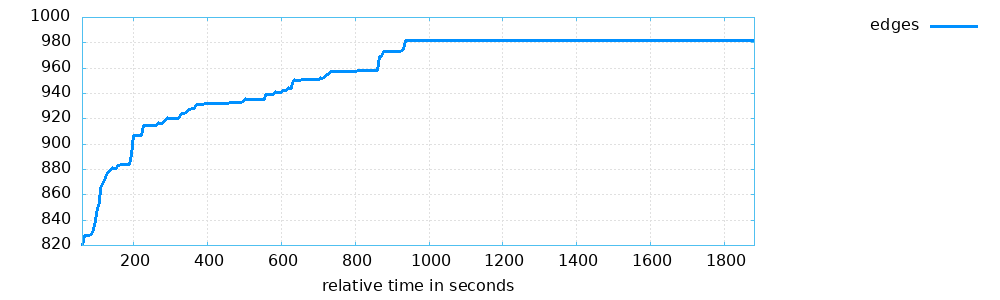
\includegraphics[width=\columnwidth]{figures/whitebox_edges.png}
    \caption{Edge discovery over time, instrumented white-box campaign
             (30~min). Steep early growth, flattens to a plateau around
             $t \approx 900$\,s: only one new edge is found in the
             final 500\,s.}
    \label{fig:wb-edges}
  \end{figure}

  \begin{figure}[H]
    \centering
    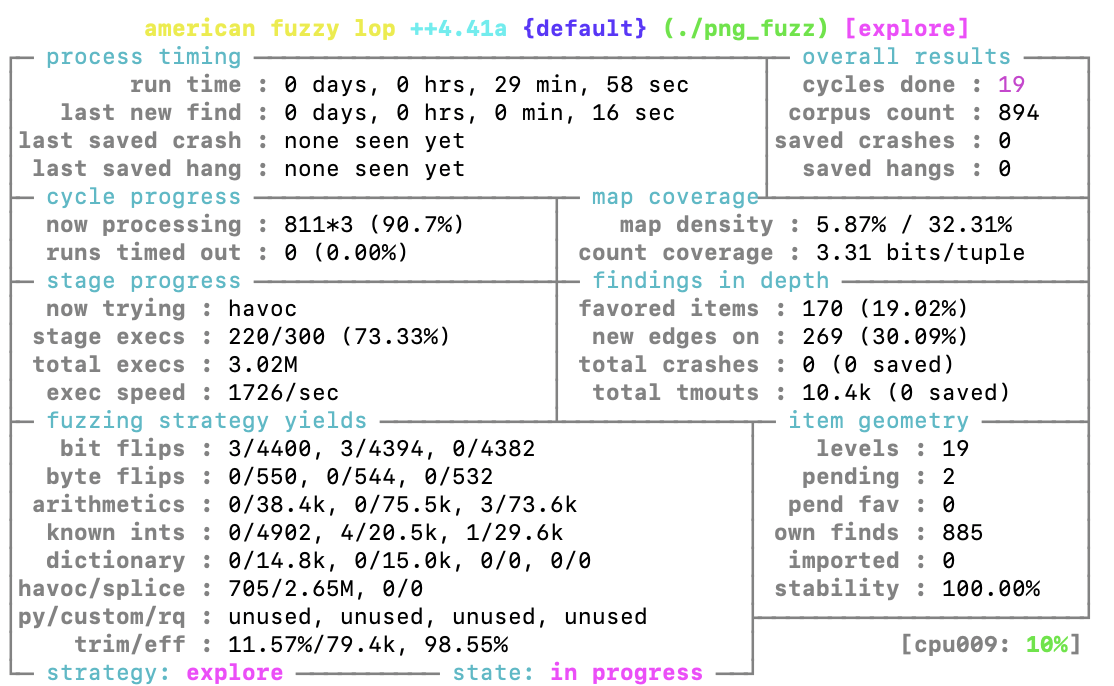
\includegraphics[width=\columnwidth]{figures/whitebox_status.png}
    \caption{Final AFL++ status screen, instrumented white-box campaign:
             19 cycles, 894 corpus entries, 1{,}002 edges (32.31\% map
             density), 100\% stability, 1{,}676\,exec/s.}
    \label{fig:wb-status}
  \end{figure}

   \begin{figure}[H]
    \centering
    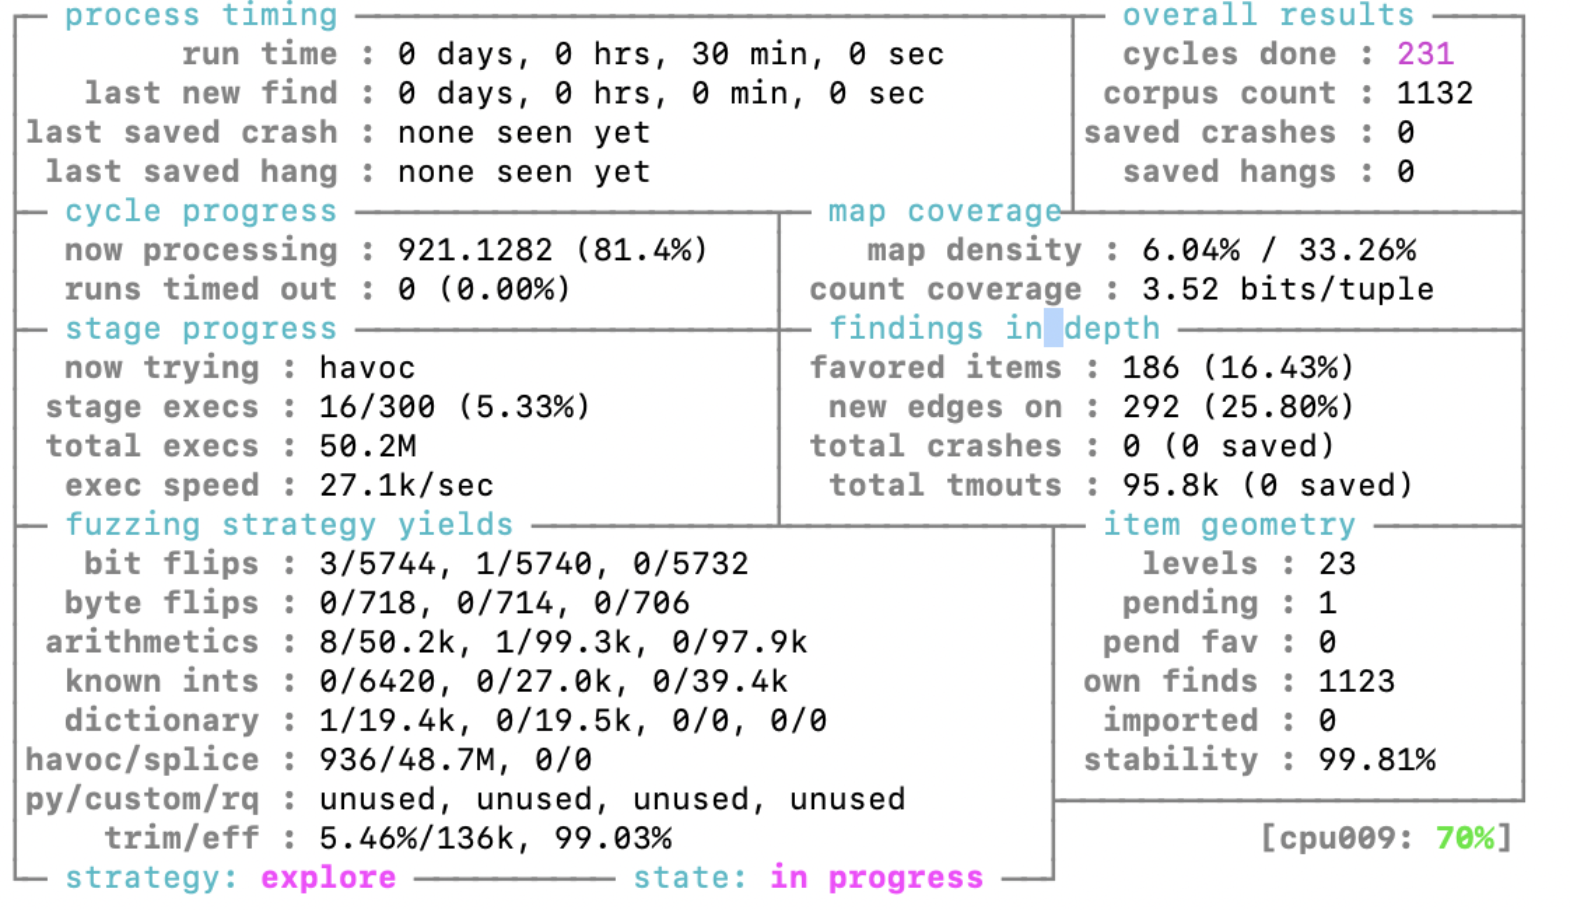
\includegraphics[width=\columnwidth]{figures/persistent_status.png}
    \caption{AFL++ status screen, white-box persistent-mode campaign:
             231 cycles, 1{,}132 corpus entries, 1{,}103 edges
             (33.26\% map density), 99.81\% stability,
             27{,}100\,exec/s, havoc: 936 new paths.}
    \label{fig:persistent-status}
  \end{figure}
  
  \begin{figure}[H]
    \centering
    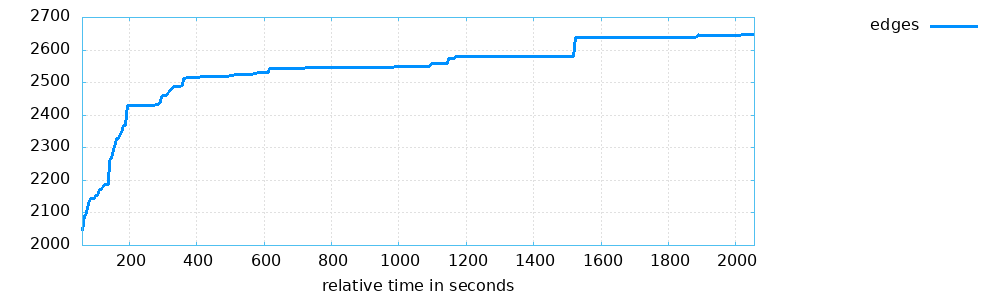
\includegraphics[width=\columnwidth]{figures/qemu_edges.png}
    \caption{Edge discovery over time, QEMU campaign (34~min).
             Coverage saturates around $t \approx 400$\,s.}
    \label{fig:qemu-edges}
  \end{figure}

  \begin{figure}[H]
    \centering
    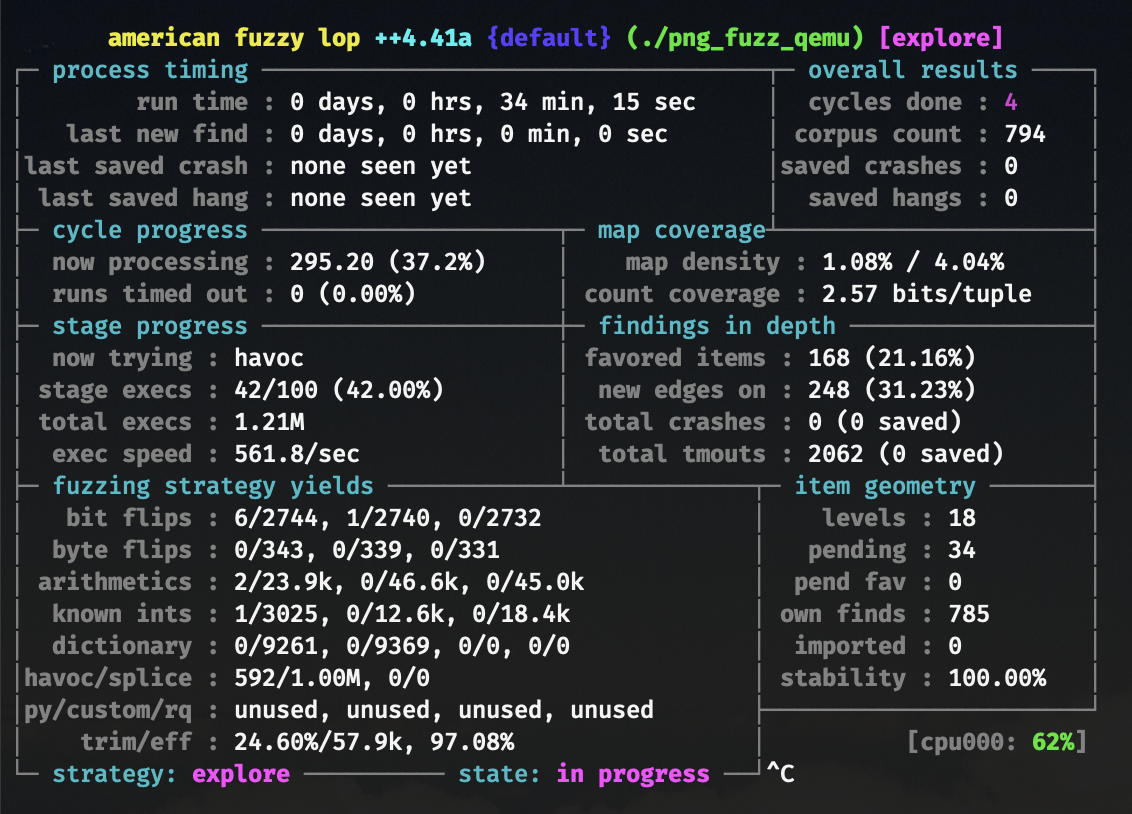
\includegraphics[width=\columnwidth]{figures/qemu_status.png}
    \caption{AFL++ status screen, QEMU campaign.}
    \label{fig:qemu-status}
  \end{figure}

  \begin{figure}[H]
    \centering
    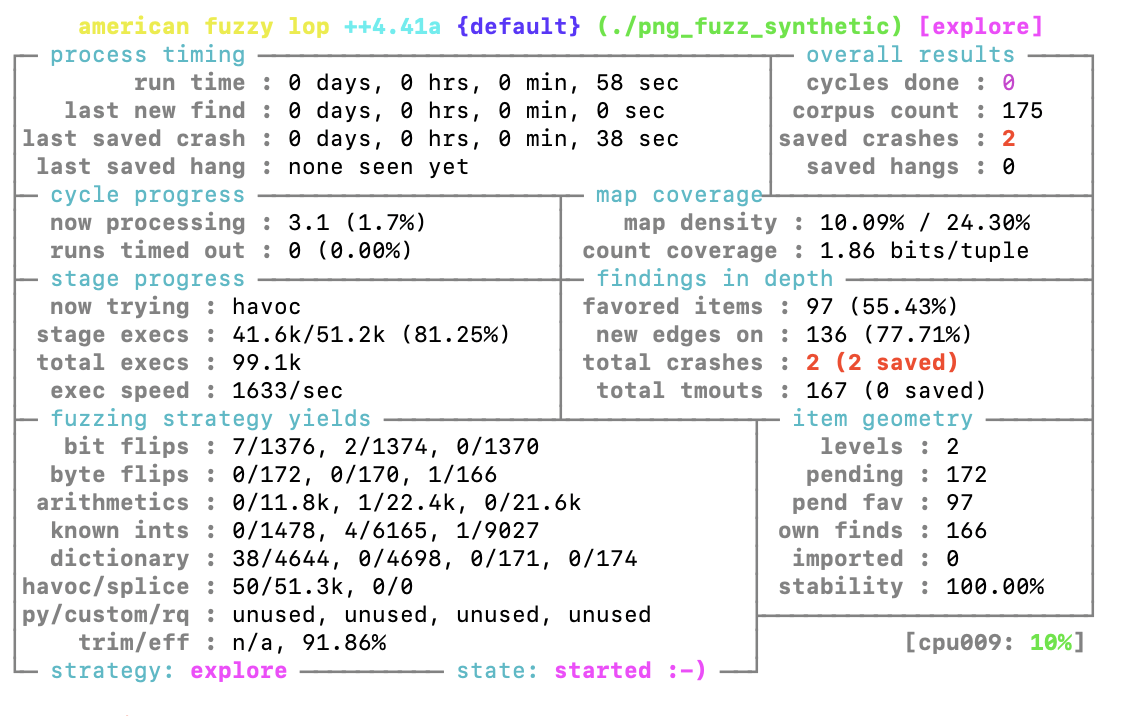
\includegraphics[width=\columnwidth]{figures/afl_synthetic.png}
    \caption{AFL++ status screen, 60-second synthetic campaign:
             2 crashes saved at $t = 38$\,s, 175 corpus entries,
             1{,}633\,exec/s, dictionary: 38 new paths.}
    \label{fig:afl-synthetic}
  \end{figure}


  \begin{figure}[H]
    \centering
    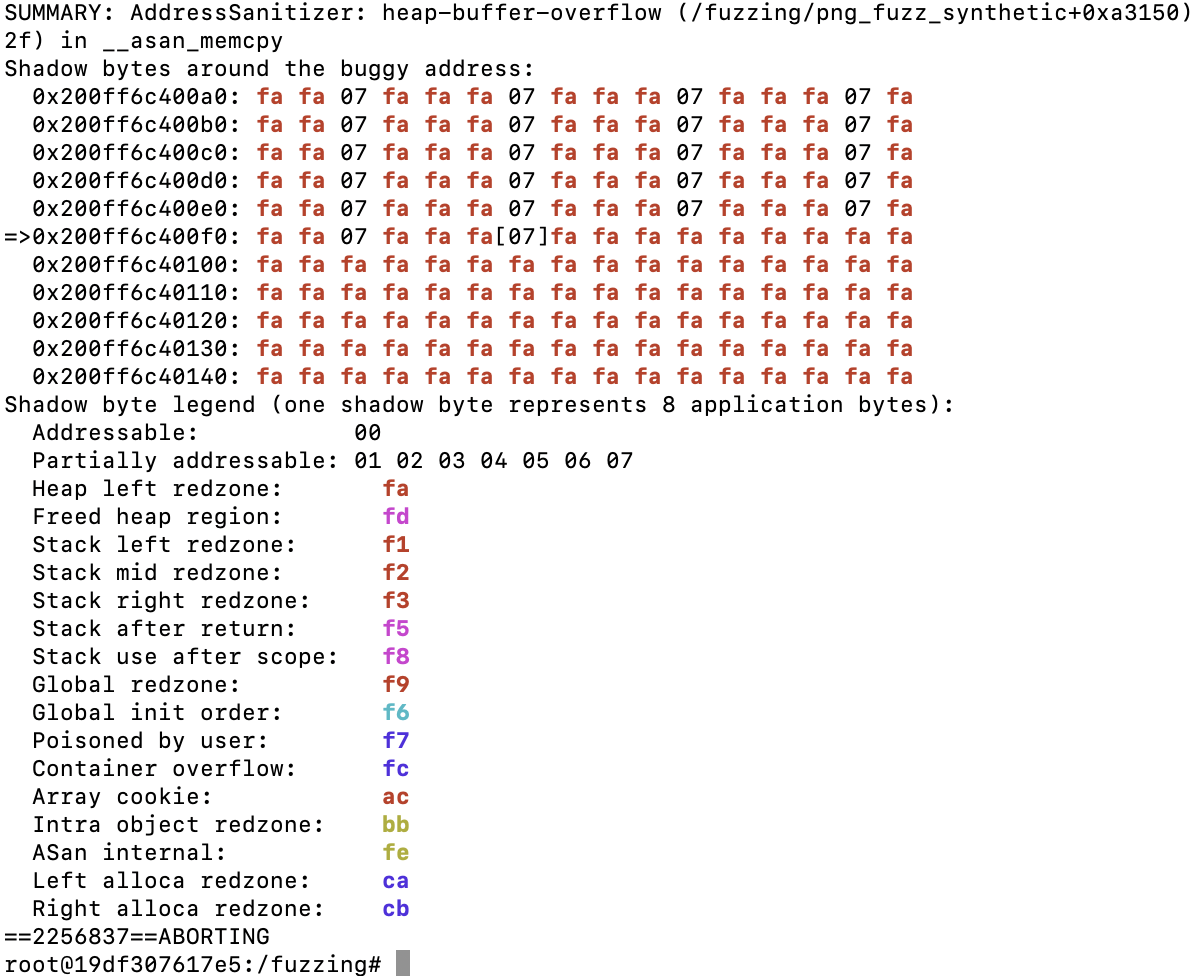
\includegraphics[width=\columnwidth]{figures/asan_synthetic.png}
    \caption{ASan output for the synthetic crash:
             \texttt{heap-buffer-overflow} in \texttt{\_\_asan\_memcpy}
             inside \texttt{png\_read\_image}.}
    \label{fig:asan-synthetic}
  \end{figure}


\clearpage
\nocite{*}
{\small
\begin{thebibliography}{12}

  \bibitem{cve}
  NIST, ``CVE-2016-10087,'' 2017.
  \url{https://nvd.nist.gov/vuln/detail/CVE-2016-10087}

  \bibitem{libpng}
  G. Randers-Pehrson et al., ``libpng Manual.''
  \url{http://www.libpng.org/pub/png/libpng-manual.txt}

  \bibitem{pngspec}
  PNG Development Group, ``PNG Specification Version 1.2.''
  \url{http://www.libpng.org/pub/png/spec/1.2/PNG-Contents.html}

  \bibitem{srlabs}
  SRLabs, ``A Beginner's Guide to Writing a Fuzzing Harness.''
  \url{https://srlabs.de/blog/guide-to-writing-fuzzing-harness}

  \bibitem{liveoverflow1}
  LiveOverflow, ``How Fuzzing with AFL works!,'' YouTube, 2021.
  \url{https://www.youtube.com/watch?v=COHUWuLTbdk}

  \bibitem{liveoverflow2}
  LiveOverflow, ``Finding Buffer Overflow with Fuzzing,'' YouTube, 2021.
  \url{https://www.youtube.com/watch?v=Do1Ri8TCF0Q}

  \bibitem{qemuyoutube}
  ``Blackbox Fuzzing using AFL++ QEMU mode,'' YouTube.
  \url{https://www.youtube.com/watch?v=sjLFf9q2NRc}

  \bibitem{aflppdocs}
  AFL++ Contributors, ``Fuzzing Binary-Only Targets.''
  \url{https://aflplus.plus/docs/fuzzing_binary-only_targets/}

  \bibitem{pillow}
  Pillow Contributors, ``Pillow Documentation.''
  \url{https://pillow.readthedocs.io/en/stable/handbook/overview.html}

  \bibitem{chromesandbox}
  The Chromium Authors, ``Chromium Sandbox Design.''
  \url{https://chromium.googlesource.com/chromium/src/+/HEAD/docs/design/sandbox.md}

  \bibitem{chromelibpng}
  Chrome Security Team, ``Q3 2025 Summary from Chrome Security,'' 2025.
  \url{https://groups.google.com/a/chromium.org/g/security-dev/c/s-UR_4pJvOY}

  \bibitem{claude}
  Anthropic, "claude-sonnet-4-6", AI assistant used for report
  writing and global review.
  \url{https://claude.ai}

  

  \end{thebibliography}
  }
  
%%%%%%%%%%%%%%%%%%%%%%%%%%%%%%%%%%%%%%%%%%%%%%%%%%%%%%%%%%%%%%%%%%%%%%%%%%%%%%%%
\end{document}
%%%%%%%%%%%%%%%%%%%%%%%%%%%%%%%%%%%%%%%%%%%%%%%%%%%%%%%%%%%%%%%%%%%%%%%%%%%%%%%%

%%  LocalWords:  endnotes includegraphics fread ptr nobj noindent
%%  LocalWords:  pdflatex acks
